\documentclass[12pt]{article}
\title{ECE M16 Homework 2}
\usepackage{subcaption}
\author{Lawrence Liu}
\usepackage{graphicx}
\usepackage[english,shorthands=off]{babel}        % shorhands=off is required for babel french in combination with tikz karnaugh....
\usepackage[utf8x]{inputenc}
\usepackage[T1]{fontenc}
\usepackage{amsmath}
\usepackage{geometry}
\geometry{verbose,a4paper, tmargin=3.5cm,bmargin=3.5cm,lmargin=2.5cm,rmargin=2.5cm,headsep=1cm,footskip=1.5cm}
\usepackage{colortbl}
\usepackage[dvipsnames]{xcolor}
\usepackage{tikz -timing}
\usepackage{tikz}
\usetikzlibrary{karnaugh}

\definecolor{LogisimKMapColor0}{RGB}{128,0,0}
\definecolor{LogisimKMapColor1}{RGB}{230,25,75}
\definecolor{LogisimKMapColor2}{RGB}{250,190,190}
\definecolor{LogisimKMapColor3}{RGB}{170,110,40}
\definecolor{LogisimKMapColor4}{RGB}{245,130,48}
\definecolor{LogisimKMapColor5}{RGB}{255,215,180}
\definecolor{LogisimKMapColor6}{RGB}{128,128,0}
\definecolor{LogisimKMapColor7}{RGB}{255,255,25}
\definecolor{LogisimKMapColor8}{RGB}{210,245,60}
\definecolor{LogisimKMapColor9}{RGB}{0,0,128}
\definecolor{LogisimKMapColor10}{RGB}{145,30,180}
\definecolor{LogisimKMapColor11}{RGB}{60,180,175}
\definecolor{LogisimKMapColor12}{RGB}{0,130,203}
\definecolor{LogisimKMapColor13}{RGB}{230,190,255}
\definecolor{LogisimKMapColor14}{RGB}{170,255,195}
\definecolor{LogisimKMapColor15}{RGB}{240,50,230}


\begin{document}
\maketitle
\section*{HW1 Problem  4 part b}
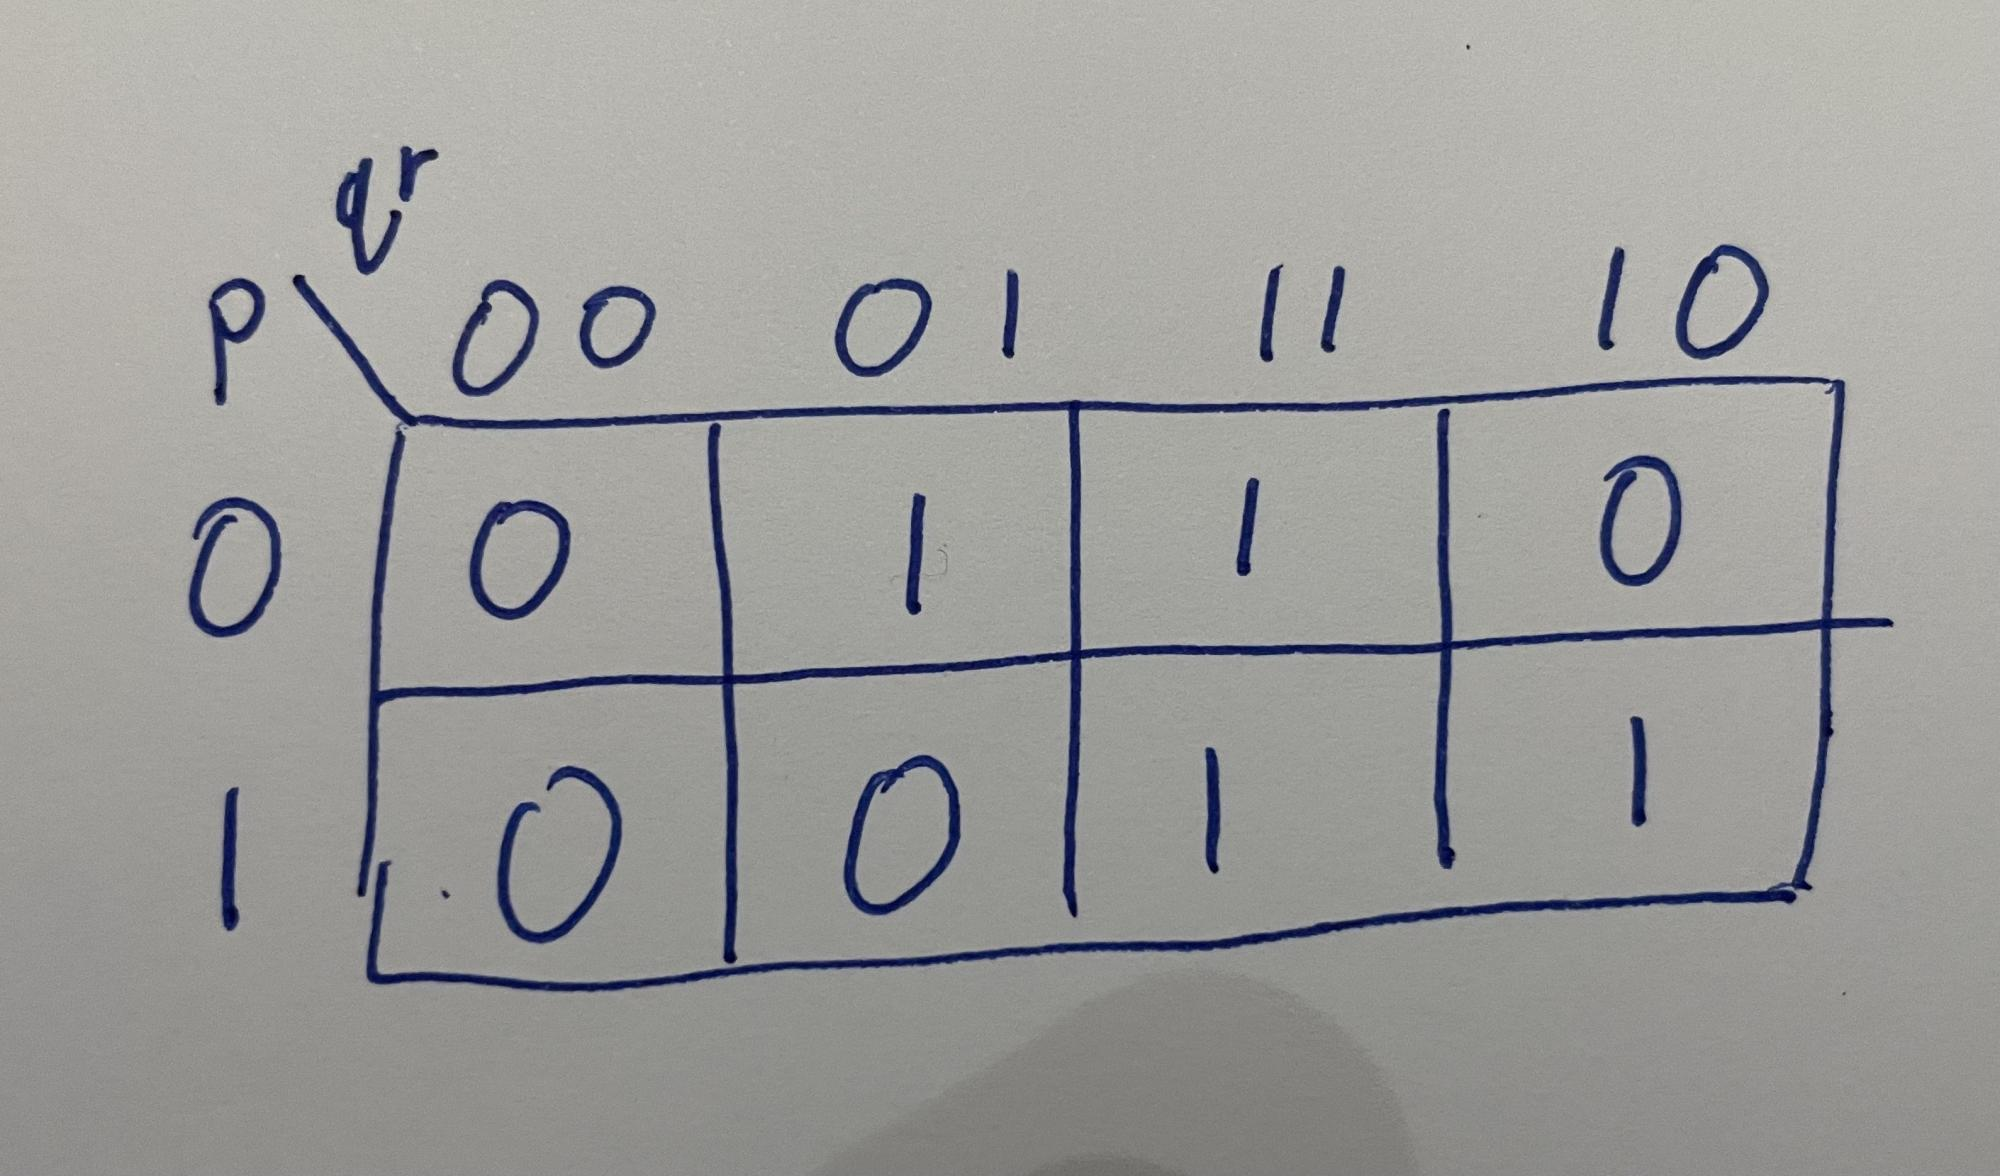
\includegraphics[scale=0.15]{../HW1/Kmap.jpg}
\section*{HW1 Problem 7}
\subsection*{(a)}
\begin{center}
    \begin{tabular}{|c|c|c|c|c|c|}
        Month & m3 & m2 & m1 & m0 & output \\
        \hline
        1 & 0 & 0 & 0 & 1 & 1 \\
        \hline
        2 & 0 & 0 & 1 & 0 & 0 \\
        \hline
        3 & 0 & 0 & 1 & 1 & 1 \\
        \hline
        4 & 0 & 1 & 0 & 0 & 0 \\
        \hline
        5 & 0 & 1 & 0 & 1 & 1 \\
        \hline
        6 & 0 & 1 & 1 & 0 & 0 \\
        \hline
        7 & 0 & 1 & 1 & 1 & 1 \\
        \hline
        8 & 1 & 0 & 0 & 0 & 1 \\
        \hline
        9 & 1 & 0 & 0 & 1 & 0 \\
        \hline
        10 & 1 & 0 & 1 & 0 & 1 \\
        \hline
        11 & 1 & 0 & 1 & 1 & 0 \\
        \hline
        12 & 1 & 1 & 0 & 0 & 1 \\
        \hline
    \end{tabular}
\end{center}
\subsection*{(b)}
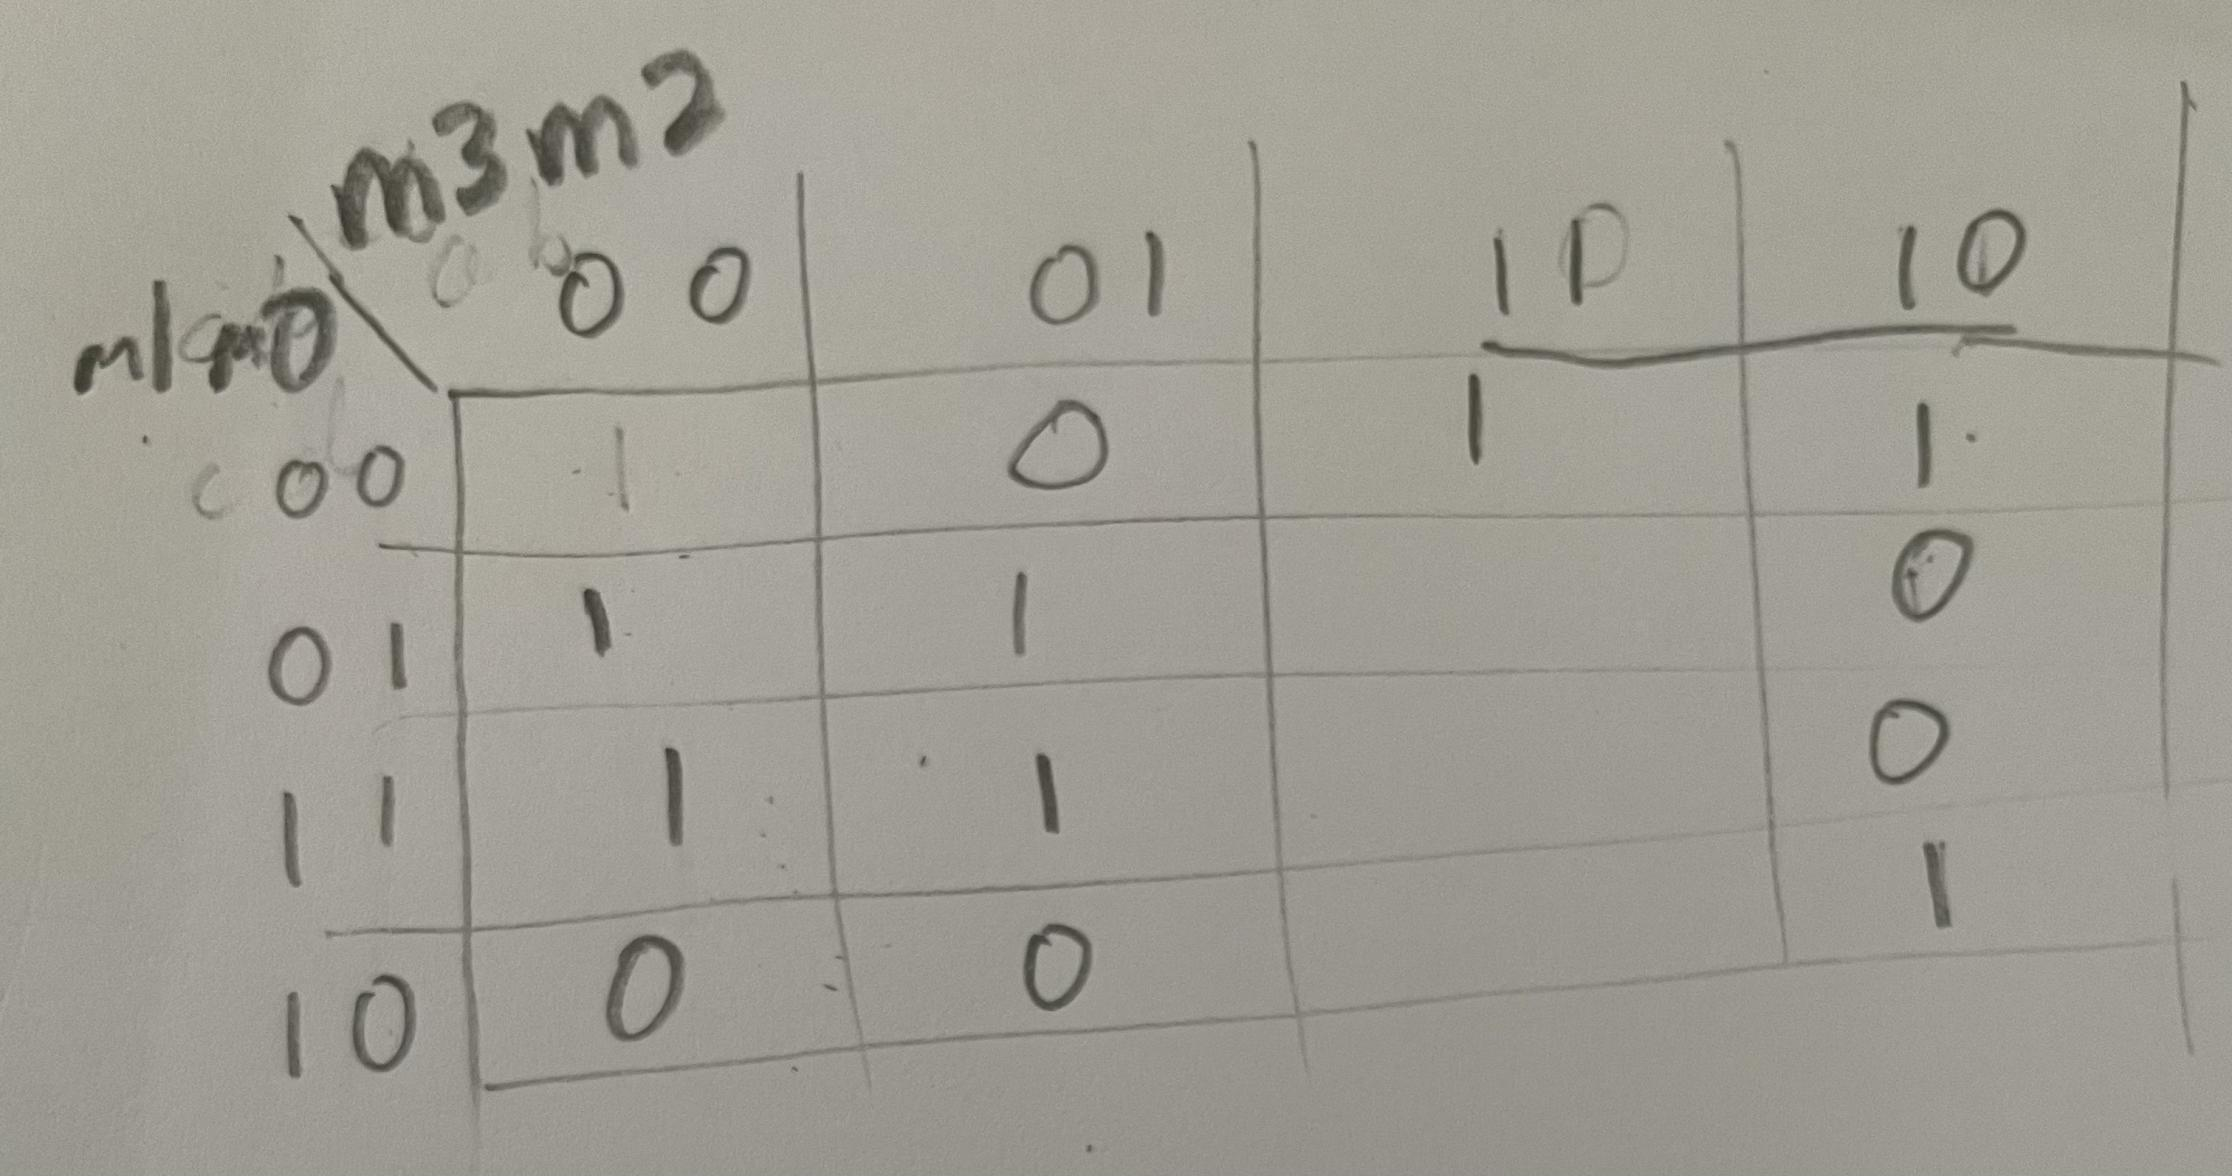
\includegraphics[scale=0.15]{Problem7Kmap.jpg}\\
Therefore the equation is:
$$\boxed{m_0.\overline{m_3}+\overline{m_0}.m3}$$
\subsection*{(c)}
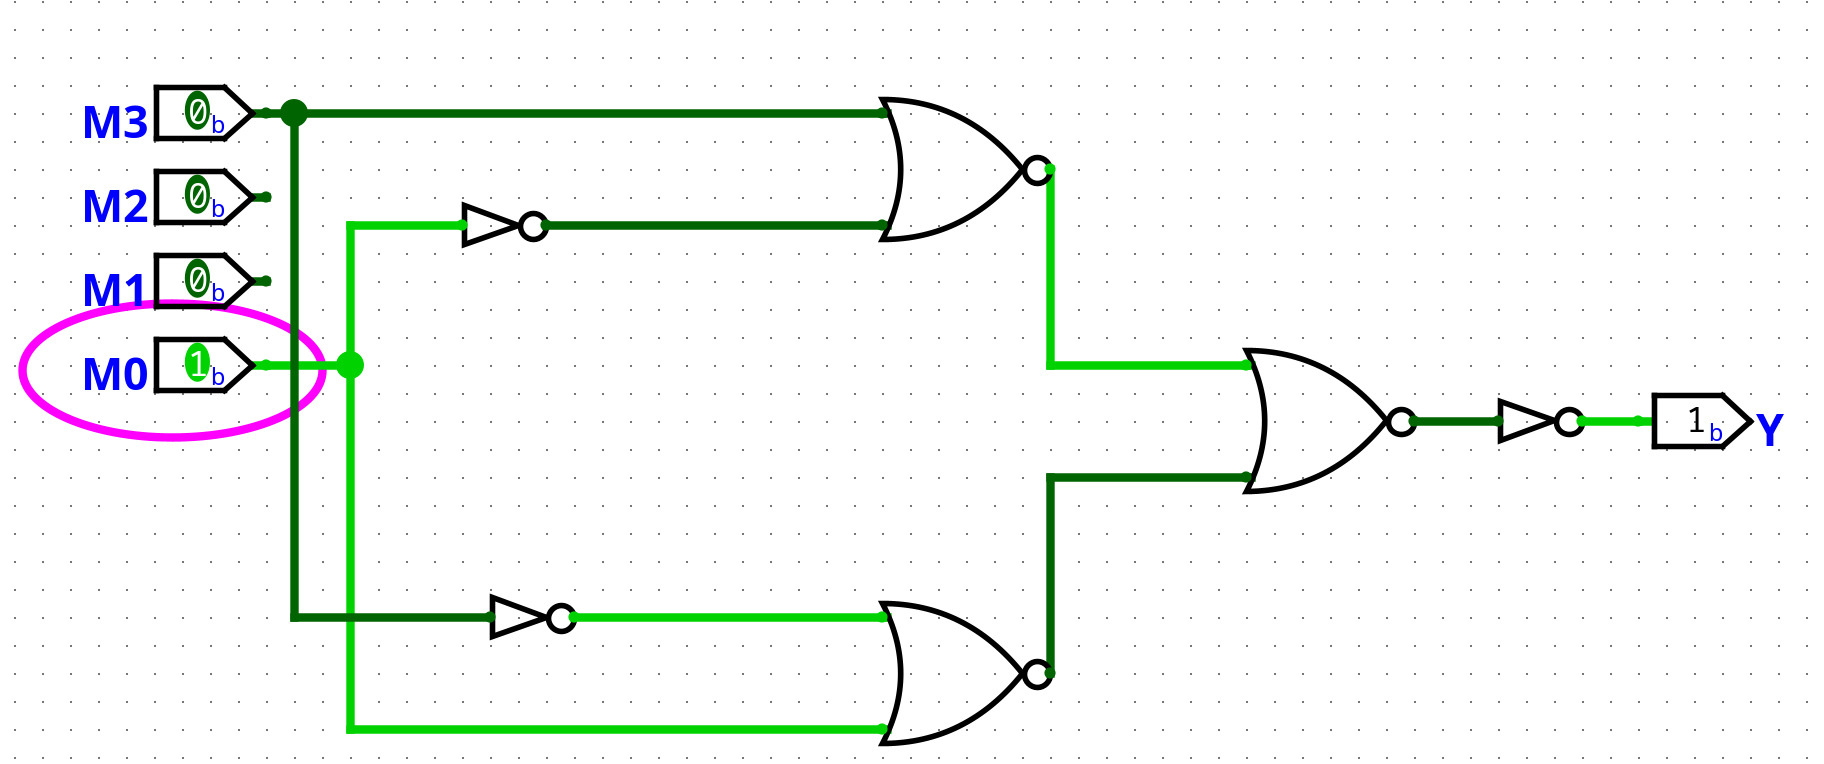
\includegraphics[scale=0.25]{Problem7Partc.png}
\section*{HW 2 Problem 1}
There would be a static 0 hazard between $b=1$, $c=1$ $a=0$ and $b=1$, $c=1$ $a=1$. We can fix it with the following circuit
We can fix this by adding an And gate between $b$ and $c$ before the nor, so the resulting function would look like this
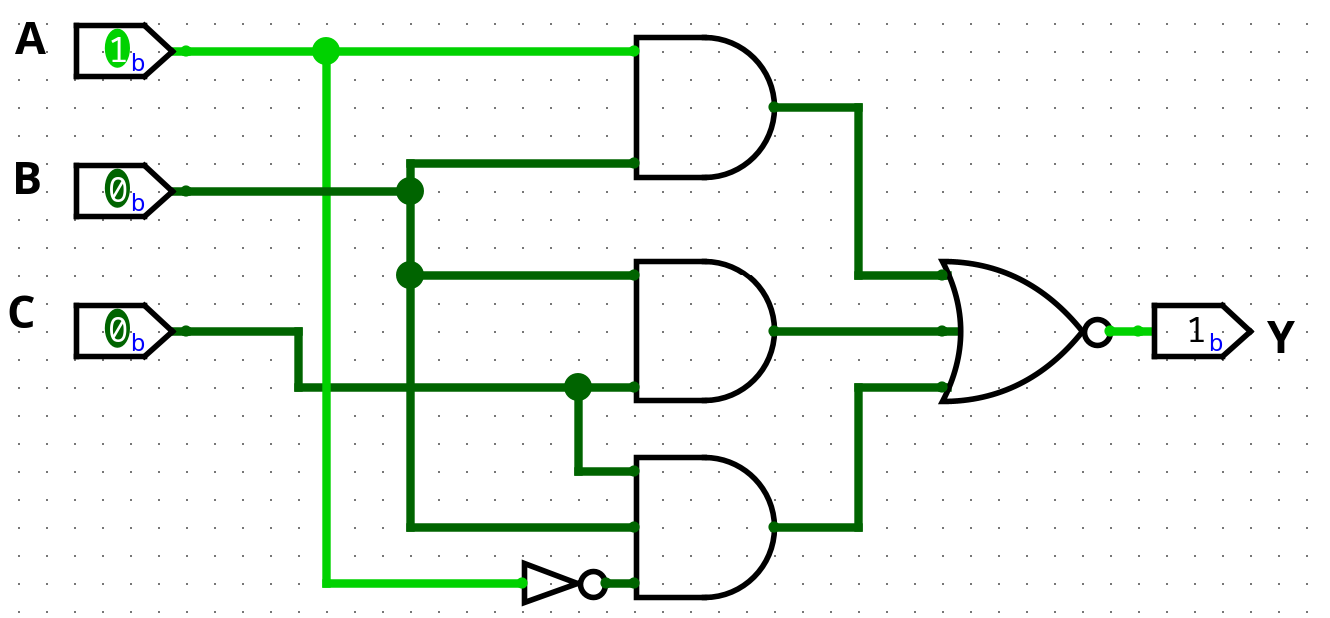
\includegraphics[scale=0.25]{Problem1.png}
\section*{Problem 2}
Let the inputs be $M[0:3]$ then we have the following truth table
\begin{center}
    \begin{tabular}{|c|c|c|c|c||c|c|}
        decimal & M3 & M2 & M1 & M0 & q2 & q5\\
        \hline
        0 & 0 & 0 & 0 & 0 & 1 & 1 \\
        \hline
        1 & 0 & 0 & 0 & 1 & 0 & 1 \\
        \hline
        2 & 0 & 0 & 1 & 0 & 1 & 1 \\
        \hline
        3 & 0 & 0 & 1 & 1 & 0 & 1 \\
        \hline
        4 & 0 & 1 & 0 & 0 & 0 & 1 \\
        \hline
        5 & 0 & 1 & 0 & 1 & 0 & 0 \\
        \hline
        6 & 0 & 1 & 1 & 0 & 1 & 0 \\
        \hline
        7 & 0 & 1 & 1 & 1 & 0 & 1 \\
        \hline
        8 & 1 & 0 & 0 & 0 & 1 & 1 \\
        \hline
        9 & 1 & 0 & 0 & 1 & 0 & 1 \\
        \hline
    \end{tabular}
\end{center}
Therefore we will have the following Kmap for q2
\begin{center}
    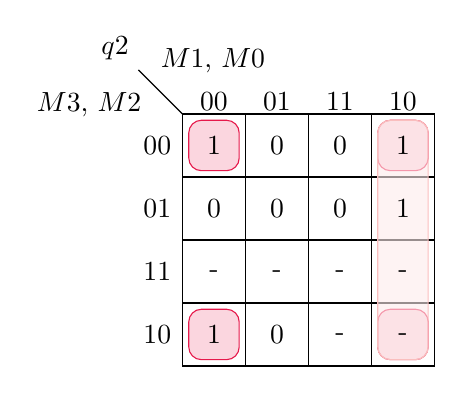
\begin{tikzpicture}[karnaugh,disable bars,x=1\kmunitlength,y=1\kmunitlength,kmbar left sep=1\kmunitlength,grp/.style n args={4}{#1,fill=#1!30,minimum width= #2\kmunitlength,minimum height=#3\kmunitlength,rounded corners=0.2\kmunitlength,fill opacity=0.6,rectangle,draw}]
    \karnaughmap{4}{$q2$}{{$M3$}{$M1$}{$M2$}{$M0$}}
    {1000101010------}{
    \draw[kmbox] (-0.5,4.5)
       node[below left]{$M3$, $M2$}
       node[above right]{$M1$, $M0$} +(-0.2,0.2)
       node[above left]{$q2$};\draw (0,4) -- (-0.7,4.7);
    \foreach \x/\1 in %
    {0/00,1/01,2/11,3/10} {
       \node at (\x+0.5,4.2) {\1};
    }
    \foreach \y/\1 in %
    {0/00,1/01,2/11,3/10} {
       \node at (-0.4,-0.5-\y+4) {\1};
    }
       \node[grp={LogisimKMapColor1}{0.8}{0.8}](n0) at(0.5,3.5) {};
       \node[grp={LogisimKMapColor1}{0.8}{0.8}](n1) at(3.5,3.5) {};
       \node[grp={LogisimKMapColor1}{0.8}{0.8}](n2) at(0.5,0.5) {};
       \node[grp={LogisimKMapColor1}{0.8}{0.8}](n3) at(3.5,0.5) {};
       \node[grp={LogisimKMapColor2}{0.8}{3.8}](n4) at(3.5,2) {};
    }
    \end{tikzpicture}
\end{center}
Therefore the equation for q2 is:
$$q2 =  \overline{M2}  \cdot  \overline{M0} +M1 \cdot  \overline{M0} $$
Likewise, the Kmap for q5 is 
\begin{center}
    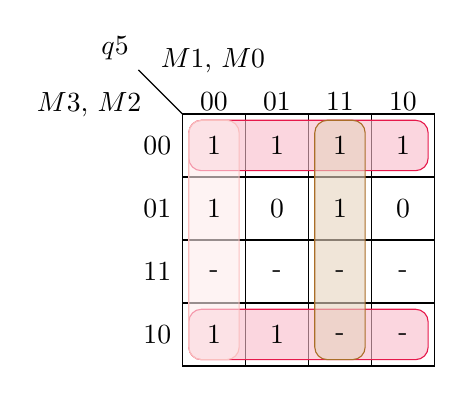
\begin{tikzpicture}[karnaugh,disable bars,x=1\kmunitlength,y=1\kmunitlength,kmbar left sep=1\kmunitlength,grp/.style n args={4}{#1,fill=#1!30,minimum width= #2\kmunitlength,minimum height=#3\kmunitlength,rounded corners=0.2\kmunitlength,fill opacity=0.6,rectangle,draw}]
    \karnaughmap{4}{$q5$}{{$M3$}{$M1$}{$M2$}{$M0$}}
    {1110110111------}{
    \draw[kmbox] (-0.5,4.5)
       node[below left]{$M3$, $M2$}
       node[above right]{$M1$, $M0$} +(-0.2,0.2)
       node[above left]{$q5$};\draw (0,4) -- (-0.7,4.7);
    \foreach \x/\1 in %
    {0/00,1/01,2/11,3/10} {
       \node at (\x+0.5,4.2) {\1};
    }
    \foreach \y/\1 in %
    {0/00,1/01,2/11,3/10} {
       \node at (-0.4,-0.5-\y+4) {\1};
    }
       \node[grp={LogisimKMapColor1}{3.8}{0.8}](n0) at(2,3.5) {};
       \node[grp={LogisimKMapColor1}{3.8}{0.8}](n1) at(2,0.5) {};
       \node[grp={LogisimKMapColor2}{0.8}{3.8}](n2) at(0.5,2) {};
       \node[grp={LogisimKMapColor3}{0.8}{3.8}](n3) at(2.5,2) {};
    }
    \end{tikzpicture}
\end{center}
Therefore the equation for q5 is:
$$q5 =  \overline{M2} + \overline{M1}  \cdot  \overline{M0} +M1 \cdot M0$$
Therefore the resulting circuit is \\
\begin{center}
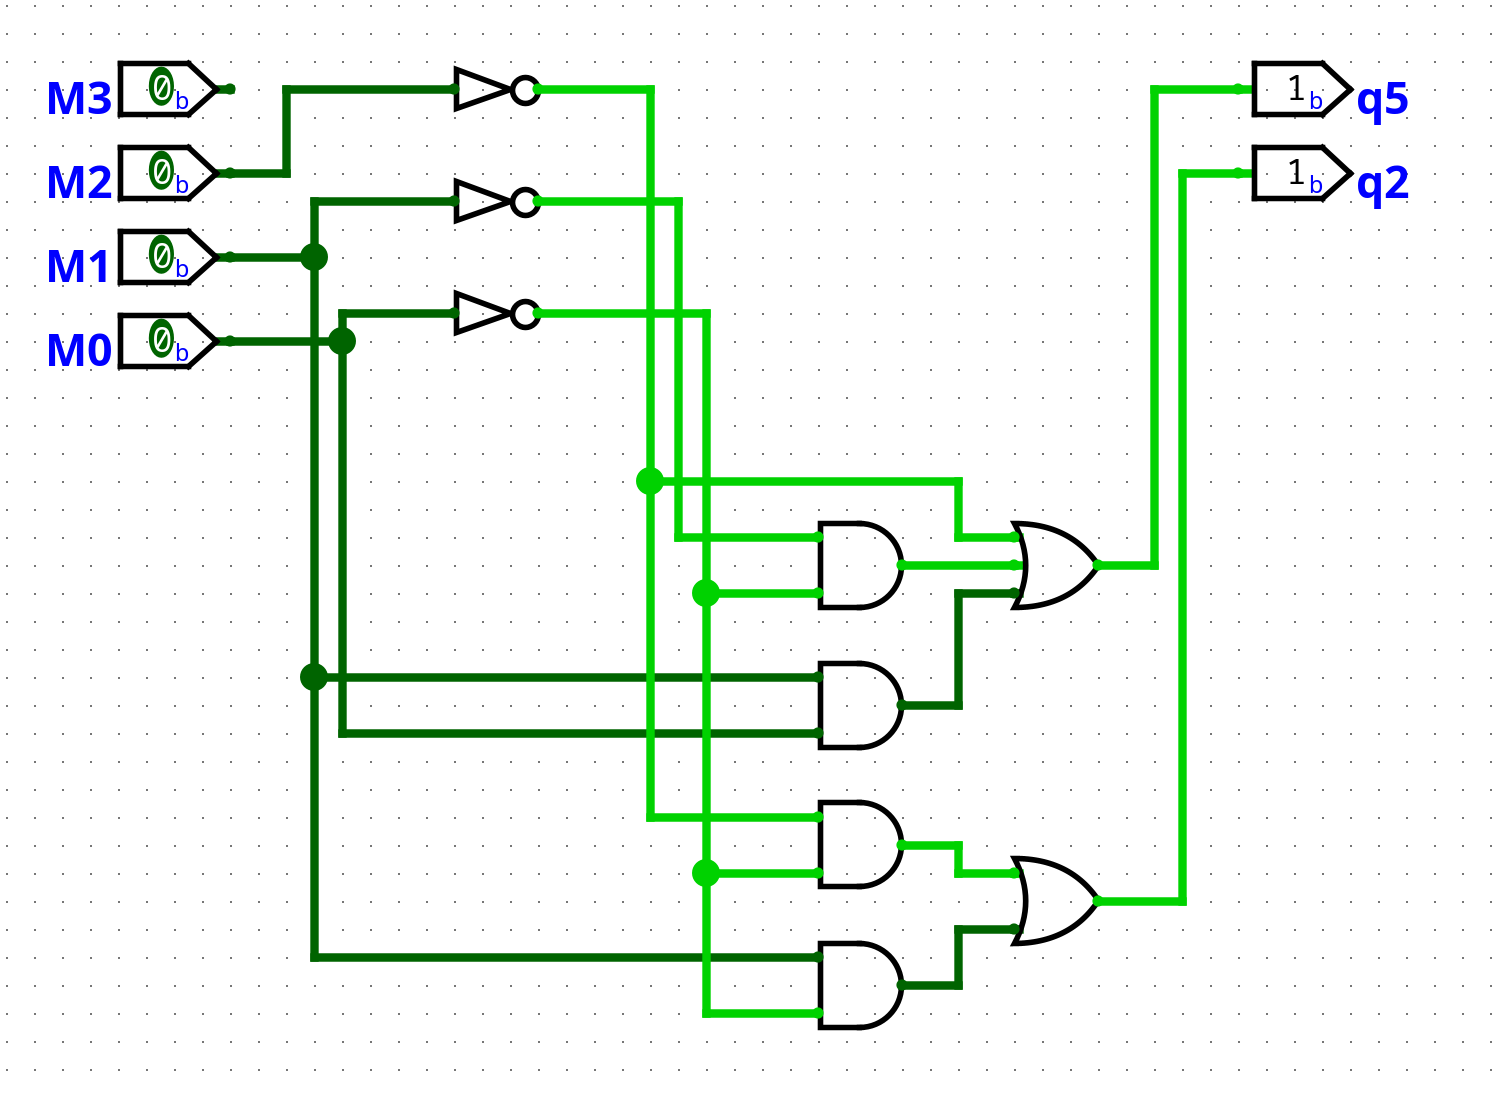
\includegraphics[scale=0.25]{Problem2.png}    
\end{center}
\end{document}